\chapter{Matchings}

\tikzset{vtx/.style={circle,fill=black,inner sep=1.6pt},
  medge/.style={line width=2.2pt}}

The last topic of the course is matchings: pairing up vertices along edges. The main results
are K\"onig's theorem (in bipartite graphs, a maximum matching and a minimum cover have the same
size) and Hall's theorem (when a bipartite graph has a matching saturating one side), together
with an algorithm that finds both a maximum matching and a certificate of optimality.

\section{Matchings and covers}

\begin{definition}[Matching]
A \emph{matching} in $G$ is a set $M$ of edges of $G$, no two of which share an end. A vertex
incident with an edge of $M$ is \emph{saturated} by $M$; otherwise it is \emph{unsaturated} (or
exposed). A \emph{perfect matching} saturates every vertex, i.e.\ $2\abs{M} = \abs{V(G)}$. A
\emph{maximum matching} is one with the largest possible number of edges.
\end{definition}

Since the edges of a matching have $2\abs{M}$ distinct ends, $2\abs{M} \le \abs{V(G)}$ always. In
particular a graph with an odd number of vertices has no perfect matching. The empty set is
always a matching, so an empty graph has only the empty matching (which is perfect only if there
are no vertices).

\begin{definition}[Cover]
A \emph{cover} of $G$ is a set $C$ of vertices such that every edge of $G$ has at least one end
in $C$. A \emph{minimum cover} is one of smallest size.
\end{definition}

\begin{lemma}
If $M$ is a matching and $C$ is a cover of $G$, then $\abs{M} \le \abs{C}$.
\end{lemma}
\begin{proof}
Each edge $e \in M$ has an end in $C$; choose one and call it $\phi(e)$. If $e \ne e'$ in $M$
then $e$ and $e'$ share no end, so $\phi(e) \ne \phi(e')$. Thus $\phi : M \to C$ is injective
and $\abs{M}\le\abs{C}$.
\end{proof}

\begin{corollary}
If $\abs{M} = \abs{C}$ for a matching $M$ and a cover $C$, then $M$ is a maximum matching and $C$
is a minimum cover.
\end{corollary}
\begin{proof}
For any matching $M'$, $\abs{M'} \le \abs{C} = \abs{M}$, so $M$ is maximum. For any cover $C'$,
$\abs{C'} \ge \abs{M} = \abs{C}$, so $C$ is minimum.
\end{proof}

So a cover of the same size is a \emph{certificate} that a matching is maximum.

\begin{example}
\begin{center}
\begin{tabular}{lcc}
\toprule
Graph & max matching & min cover\\
\midrule
$C_n$ & $\floor{n/2}$ & $\ceil{n/2}$\\
$K_n$ & $\floor{n/2}$ & $n - 1$\\
$K_{p,q}$, $p \le q$ & $p$ & $p$\\
\bottomrule
\end{tabular}
\end{center}
For $K_n$: if a set misses two vertices $u, v$, the edge $uv$ is uncovered, so a cover has at
least $n - 1$ vertices. For odd cycles and complete graphs the two numbers differ, so the
inequality $\abs{M}\le\abs{C}$ can be strict in general.
\end{example}

\section{Augmenting paths}

\begin{definition}[Alternating and augmenting paths]
Let $M$ be a matching. An \emph{$M$-alternating path} is a path whose edges alternate between
not in $M$ and in $M$. An \emph{$M$-augmenting path} is an alternating path with at least one edge
whose two ends are both unsaturated by $M$.
\end{definition}

An augmenting path has odd length, and its first and last edges are not in $M$; it has one more
non-matching edge than matching edges.

\begin{lemma}
If $M$ has an augmenting path $P$, then $M$ is not a maximum matching.
\end{lemma}
\begin{proof}
Let $M' = M \triangle E(P)$: remove the edges of $P$ that are in $M$ and add those that are not.
Internal vertices of $P$ were matched by one edge of $P$ and are now matched by the other; the two
ends were unsaturated and are now matched by one edge of $P$; vertices off $P$ are unaffected. So
$M'$ is a matching, with $\abs{M'} = \abs{M} + 1$.
\end{proof}

\begin{center}
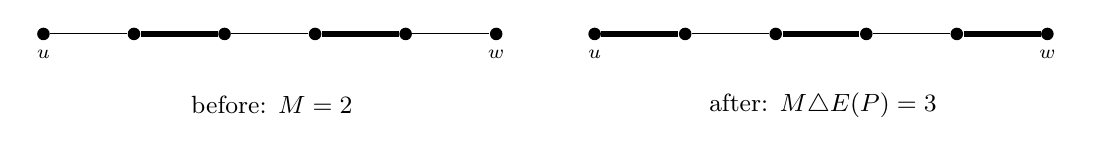
\begin{tikzpicture}[every label/.style={font=\scriptsize}]
  \foreach \s/\title in {0/{before: $\abs{M} = 2$},1/{after: $\abs{M \triangle E(P)} = 3$}} {
    \begin{scope}[xshift=\s*7cm]
      \foreach \i/\l in {0/u,1/{},2/{},3/{},4/{},5/w} {
        \node[vtx,label=below:$\l$] (p\s\i) at (1.15*\i,0) {};
      }
      \node[font=\small] at (2.9,-0.9) {\title};
    \end{scope}
  }
  \draw (p00)--(p01) (p02)--(p03) (p04)--(p05);
  \draw[medge] (p01)--(p02) (p03)--(p04);
  \draw[medge] (p10)--(p11) (p12)--(p13) (p14)--(p15);
  \draw (p11)--(p12) (p13)--(p14);
\end{tikzpicture}
\end{center}
An augmenting path from the unsaturated vertex $u$ to the unsaturated vertex $w$: swapping
matching (thick) and non-matching edges along it gains one edge.

\begin{theorem}[Berge]
A matching $M$ is maximum if and only if there is no $M$-augmenting path.
\end{theorem}
\begin{proof}[Proof sketch]
One direction is the lemma. Conversely, if $M^*$ is a matching with $\abs{M^*} > \abs{M}$, consider
the subgraph with edge set $M \triangle M^*$. Each vertex has degree at most $2$ in it, so its
components are paths and cycles whose edges alternate between $M$ and $M^*$. Cycles have equally
many edges of each; since $M^*$ has more edges overall, some path component has more $M^*$-edges
than $M$-edges, and that path is $M$-augmenting.
\end{proof}

\section{The bipartite matching algorithm}

Let $G$ be bipartite with bipartition $(A,B)$, and $M$ a matching.
\begin{important}[One round of the algorithm]
\begin{enumerate}
  \item Let $X_0$ be the set of vertices of $A$ unsaturated by $M$.
  \item Let $Z$ be the set of vertices joined to a vertex of $X_0$ by an $M$-alternating path
        (grow alternating trees from $X_0$: from $A$ follow non-matching edges to $B$, from $B$
        follow the matching edge back to $A$).
  \item If $Z$ contains an unsaturated vertex of $B$, the alternating path to it is augmenting:
        augment and start the next round.
  \item Otherwise set $X = A\cap Z$, $Y = B\cap Z$ and output $M$ and the cover
        $C = Y \cup (A \setminus X)$.
\end{enumerate}
\end{important}

\begin{lemma}
With the notation above, let $U$ be the set of unsaturated vertices in $Y$. Then
\begin{enumerate}
  \item[(a)] there is no edge from $X$ to $B\setminus Y$;
  \item[(b)] $C = Y\cup(A\setminus X)$ is a cover of $G$;
  \item[(c)] there is no edge of $M$ from $Y$ to $A \setminus X$;
  \item[(d)] $\abs{M} = \abs{C} - \abs{U}$;
  \item[(e)] there is an $M$-augmenting path to each vertex of $U$.
\end{enumerate}
\end{lemma}
\begin{proof}
(a) Suppose $uv \in E(G)$ with $u\in X$ and $v \in B\setminus Y$. There is an alternating path $P$
from $X_0$ to $u$; it has even length (it starts and ends in $A$), so it is empty or ends with a
matching edge. Then $uv \notin M$ (if $u \in X_0$ it is unsaturated; otherwise its matching edge is
the last edge of $P$, which goes to $Y$). So $P$ followed by $uv$ is an alternating path to $v$
(if $v$ is not already on $P$; but all vertices of $P$ are in $Z$, and $v \notin Z$), hence $v \in Z$,
contradicting $v \notin Y$.

(b) Every edge joins $A$ to $B$. Edges from $X$ go to $Y \subseteq C$ by (a); edges from
$A\setminus X$ have an end in $A \setminus X \subseteq C$.

(c) Suppose $vw\in M$ with $v \in A\setminus X$ and $w \in Y$. The alternating path $P$ from $X_0$
to $w$ has odd length, so its last edge is not in $M$, and $v$ is not on $P$ (the vertices of $P$
are in $Z$). Then $P$ followed by $wv$ is an alternating path to $v$, so $v \in Z \cap A = X$, a
contradiction.

(d) Every vertex of $A\setminus X$ is saturated (as $X_0 \subseteq X$), and by (c) and (a) its
matching edge goes to $B\setminus Y$. Every saturated vertex of $Y$ has its matching edge going to
$X$ by (c). These matching edges are all distinct, and every edge of $M$ is of one of these two
kinds (an edge of $M$ from $X$ goes to $Y$ by (a)). Hence
$\abs{M} = \abs{A\setminus X} + (\abs{Y} - \abs{U}) = \abs{C} - \abs{U}$.

(e) A vertex $v \in U$ is in $Z$, so there is an alternating path from an unsaturated vertex of
$X_0$ to $v$, and $v$ is unsaturated: this path is augmenting.
\end{proof}

So if the algorithm stops (no augmenting path found, i.e.\ $U = \emptyset$), (b) and (d) give a
cover $C$ with $\abs{C} = \abs{M}$, proving $M$ is maximum. Each augmentation increases $\abs{M}$,
so the algorithm terminates after at most $\abs{A}$ rounds.

\begin{example}
Let $A = \{a_1,a_2,a_3,a_4\}$, $B=\{b_1,b_2,b_3,b_4\}$ with edges
$a_1b_1$, $a_2b_1$, $a_2b_2$, $a_3b_2$, $a_4b_2$, $a_4b_3$, $a_4b_4$. Start with $M = \{a_2b_1, a_4b_2\}$.

\emph{Round 1.} $X_0 = \{a_1, a_3\}$. From $a_1$: $a_1 \to b_1$ (non-matching), $b_1 \to a_2$
(matching), $a_2 \to b_2$, $b_2 \to a_4$, $a_4 \to b_3$, and $b_3$ is unsaturated. Augment along
$a_1b_1a_2b_2a_4b_3$: the new matching is $M = \{a_1b_1, a_2b_2, a_4b_3\}$.

\emph{Round 2.} $X_0 = \{a_3\}$. From $a_3$: $a_3 \to b_2 \to a_2 \to b_1 \to a_1$, and $a_1$ has
no other neighbours. So $Z = \{a_3, b_2, a_2, b_1, a_1\}$, containing no unsaturated vertex of $B$.
Then $X = \{a_1,a_2,a_3\}$, $Y = \{b_1,b_2\}$, and
\[
C = Y \cup (A\setminus X) = \{b_1, b_2, a_4\}.
\]
Indeed $C$ covers every edge, and $\abs{C} = 3 = \abs{M}$, so $M$ is a maximum matching. There is
no perfect matching: $a_1, a_2, a_3$ have only the two neighbours $b_1, b_2$.
\begin{center}
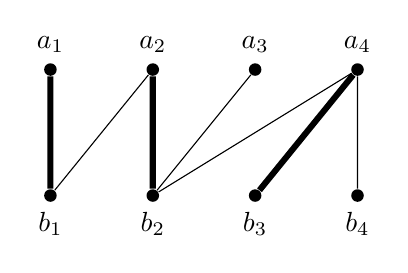
\begin{tikzpicture}
  \foreach \i in {1,...,4} {
    \node[vtx,label=above:$a_\i$] (a\i) at (1.3*\i,1.6) {};
    \node[vtx,label=below:$b_\i$] (b\i) at (1.3*\i,0) {};
  }
  \draw (a2)--(b1) (a3)--(b2) (a4)--(b2) (a4)--(b4);
  \draw[medge] (a1)--(b1) (a2)--(b2) (a4)--(b3);
\end{tikzpicture}
\end{center}
(Thick edges: the final maximum matching.)

The certificate from round 2: the cover $C = \{b_1, b_2, a_4\}$ (circled) has $3$ vertices and
touches every edge, and the set $X = \{a_1, a_2, a_3\}$ (shaded) has only the two neighbours
$b_1, b_2$, violating Hall's condition.
\begin{center}
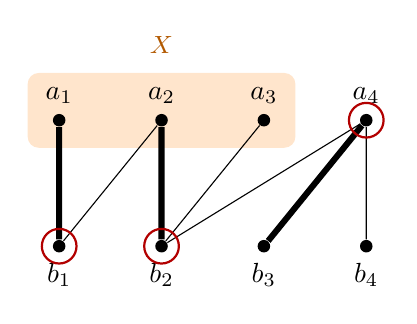
\begin{tikzpicture}
  \fill[orange!20,rounded corners] (0.9,1.25) rectangle (4.3,2.2);
  \foreach \i in {1,...,4} {
    \node[vtx,label=above:$a_\i$] (a\i) at (1.3*\i,1.6) {};
    \node[vtx,label=below:$b_\i$] (b\i) at (1.3*\i,0) {};
  }
  \draw (a2)--(b1) (a3)--(b2) (a4)--(b2) (a4)--(b4);
  \draw[medge] (a1)--(b1) (a2)--(b2) (a4)--(b3);
  \foreach \v in {b1,b2,a4} \draw[red!70!black,thick] (\v) circle (0.22);
  \node[orange!70!black,font=\small] at (2.6,2.55) {$X$};
\end{tikzpicture}
\end{center}
\end{example}

\section{K\"onig's theorem}

\begin{theorem}[K\"onig]
In a bipartite graph, the maximum size of a matching equals the minimum size of a cover.
\end{theorem}
\begin{proof}
Let $M$ be a maximum matching. By Berge's lemma there is no augmenting path, so in the algorithm
$U = \emptyset$ by (e). By (b) and (d), $C = Y \cup (A\setminus X)$ is a cover with
$\abs{C} = \abs{M}$. Combined with $\abs{M}\le\abs{C'}$ for every cover $C'$, the result follows.
\end{proof}

This fails for non-bipartite graphs: in $C_3 = K_3$ a maximum matching has $1$ edge but a minimum
cover has $2$ vertices.

\section{Hall's theorem}

For $D \subseteq V(G)$, the \emph{neighbour set} $N(D)$ is the set of vertices adjacent to at
least one vertex of $D$.

\begin{theorem}[Hall]
Let $G$ be bipartite with bipartition $(A,B)$. Then $G$ has a matching saturating every vertex of
$A$ if and only if $\abs{N(D)} \ge \abs{D}$ for every $D \subseteq A$.
\end{theorem}
\begin{proof}
($\Rightarrow$) If $M$ saturates $A$, the vertices of $D$ are matched to $\abs{D}$ distinct vertices,
all in $N(D)$.

($\Leftarrow$) Suppose there is no matching saturating $A$. Let $M$ be a maximum matching, so
$\abs{M} < \abs{A}$, and let $X, Y$ be as in the algorithm (with $U = \emptyset$). By (a), every
neighbour of $X$ lies in $Y$, so $N(X) \subseteq Y$. By (d),
$\abs{M} = \abs{Y} + \abs{A} - \abs{X}$, so $\abs{Y} = \abs{M} - \abs{A} + \abs{X} < \abs{X}$.
Thus $D = X$ satisfies $\abs{N(D)} \le \abs{Y} < \abs{D}$.
\end{proof}

In the example above, $D = \{a_1,a_2,a_3\}$ has $N(D) = \{b_1,b_2\}$, a set violating Hall's
condition; this is exactly the set $X$ the algorithm produced.

\section{Perfect matchings in bipartite graphs}

\begin{corollary}
A bipartite graph with bipartition $(A,B)$ has a perfect matching iff $\abs{A} = \abs{B}$ and
$\abs{N(D)}\ge\abs{D}$ for every $D\subseteq A$.
\end{corollary}

\begin{theorem}
Every $k$-regular bipartite graph with $k\ge1$ has a perfect matching.
\end{theorem}
\begin{proof}
Counting edges from each side, $k\abs{A} = \abs{E} = k\abs{B}$, so $\abs{A} = \abs{B}$. For
$D \subseteq A$, the $k\abs{D}$ edges incident with $D$ all end in $N(D)$, and each vertex of
$N(D)$ is incident with at most $k$ of them, so $k\abs{N(D)} \ge k\abs{D}$. By Hall, there is a
matching saturating $A$, which is perfect since $\abs{A} = \abs{B}$.
\end{proof}

\begin{corollary}
$Q_n$ has a perfect matching for $n\ge1$ (it is $n$-regular and bipartite). Applying the theorem
repeatedly (removing a perfect matching leaves a $(k-1)$-regular bipartite graph), the edges of a
$k$-regular bipartite graph split into $k$ perfect matchings, so $\chi' = k$.
\end{corollary}

\section{Systems of distinct representatives}

\begin{definition}[SDR]
Given sets $S_1, \dots, S_n$, a \emph{system of distinct representatives} is a choice of
\emph{distinct} elements $s_1, \dots, s_n$ with $s_i \in S_i$.
\end{definition}

Form the bipartite graph with $A = \{S_1,\dots,S_n\}$, $B = \bigcup S_i$, and $S_i$ adjacent to
each element it contains. An SDR is exactly a matching saturating $A$, so by Hall:

\begin{corollary}
$S_1, \dots, S_n$ have an SDR iff for every $I \subseteq [n]$,
$\abs{\bigcup_{i\in I}S_i} \ge \abs{I}$.
\end{corollary}

\begin{example}
$S_1 = \{1,2\}$, $S_2 = \{2\}$, $S_3 = \{1,2\}$, $S_4 = \{2,3,4\}$ have no SDR: $S_1\cup S_2\cup S_3 =
\{1,2\}$ has only $2$ elements for $3$ sets. Replacing $S_3$ by $\{1,3\}$ gives the SDR
$1, 2, 3, 4$.
\end{example}

\section{Summary}
\begin{itemize}
  \item $\abs{M}\le\abs{C}$ for any matching and cover; equality certifies optimality.
  \item Augmenting paths increase a matching; $M$ is maximum iff none exists (Berge).
  \item Bipartite algorithm: grow alternating paths from unsaturated $A$-vertices; either augment
        or output the cover $Y\cup(A\setminus X)$ of size $\abs{M}$.
  \item K\"onig: max matching $=$ min cover in bipartite graphs.
  \item Hall: a matching saturating $A$ exists iff $\abs{N(D)}\ge\abs{D}$ for all $D\subseteq A$;
        $k$-regular bipartite graphs have perfect matchings; SDRs.
\end{itemize}
